\documentclass[conference]{IEEEtran}
\IEEEoverridecommandlockouts

\usepackage{cite}
\usepackage{amsmath,amssymb,amsfonts}
\usepackage{graphicx}
\usepackage{textcomp}
\usepackage{xcolor}
\usepackage{booktabs}
\usepackage{microtype}
\usepackage{url}
\usepackage{balance}

% Path to graphics
\graphicspath{{figures/}}

\begin{document}

\title{SPECTRE-GRID: Mitigating Neighborhood Heterophily in Spatio-Temporal Graph Neural Networks for High-Speed Network Intrusion Detection}

\author{\IEEEauthorblockN{Abra\~ao Teixeira da Silva}
\IEEEauthorblockA{\textit{Department of Computer Science} \\
\textit{Instituto Federal Catarinense (IFC) --- Campus Brusque}\\
Brusque, Santa Catarina, Brazil \\
abraao.silva@ifc.edu.br}
\and
\IEEEauthorblockN{Jackson Mallmann}
\IEEEauthorblockA{\textit{Department of Computer Science} \\
\textit{Instituto Federal Catarinense (IFC) --- Campus Brusque}\\
Brusque, Santa Catarina, Brazil \\
jackson.mallmann@ifc.edu.br}
}

\maketitle

\begin{abstract}
Deep learning architectures for Network Intrusion Detection Systems (NIDS) predominantly rely on isolated temporal representations (e.g., 1D-CNN, LSTM), ignoring inter-host relational topology, or deploy Graph Neural Networks (GNNs) that fail to account for neighborhood heterophily in network communication graphs. In enterprise networks, communication flows are inherently asymmetric and directed: an attacking host initiates aggressive reconnaissance or denial-of-service traffic directed at benign enterprise servers. Under standard forward message passing ($src \to dst$), target victim nodes aggregate anomalous embeddings from attackers, inflating False Positive Rates (FPR) and overwhelming Security Operations Centers (SOCs). To resolve this fundamental limitation, we present \textbf{SPECTRE-GRID}, a hardware-conscious intrusion detection architecture that couples an in-kernel eBPF/XDP stateful packet extraction pipeline with a Spatio-Temporal Graph Attention Network (STGNN). We systematically formulate the topological heterophily problem and demonstrate that incorporating bidirectional message passing, edge reversal ($dst \to src$), and temporal residual skip connections effectively decouples victim representations from attacker aggression. On the UNSW-NB15 benchmark active horizon ($200{,}000$ chronological flows, $22{,}215$ attacks), bidirectional GAT achieves a validation $F_1$-score of $0.9609 \pm 0.0067$ (peak $0.9666$, weighted $0.9618$) while suppressing the validation FPR to $0.73\% \pm 0.12\%$, an $88\%$ reduction in false alarms compared to purely temporal CNN-LSTM baselines ($F_1 = 0.7516$, $\text{FPR} = 5.89\%$). To ensure scientific validity, all evaluations enforce a strict leakage-free temporal snapshot protocol ($\Delta t = 30\text{ s}$) where normalizers and feature selectors are fitted exclusively on chronological training slices. Furthermore, independent evaluation on an unseen slice of UNSW-NB15\_2 (rows $400{,}000 \dots 600{,}000$, containing $32{,}550$ attack flows) under concept drift demonstrates that while temporal-only baselines degrade to $F_1 = 0.6773$ and $\text{FPR} = 8.79\%$, SPECTRE-GRID preserves high generalization ($F_1 = 0.9167$, $\text{FPR} = 1.47\%$, with mean Precision of $0.8837$ and Recall of $0.9525$). Empirical benchmarks confirm streaming inference latencies between $3.14\text{ ms}$ and $5.42\text{ ms}$ per snapshot on consumer GPU hardware with peak VRAM below $67\text{ MiB}$, proving the computational feasibility of continuous streaming graph-level intrusion detection without queue backlog.
\end{abstract}

\begin{IEEEkeywords}
Network Intrusion Detection, eBPF/XDP, Graph Attention Networks, Spatio-Temporal Modeling, Heterophily, Data Leakage Prevention, Concept Drift.
\end{IEEEkeywords}

\section{Introduction}

The escalating complexity of contemporary cyber threats---ranging from distributed denial-of-service (DDoS) campaigns and multi-stage lateral movement to stealthy reconnaissance---has exposed the operational limitations of conventional signature-based Network Intrusion Detection Systems (NIDS)~\cite{scarfone2007guide}. To automate threat discovery, deep learning (DL) methods have been widely adopted~\cite{vinayakumar2019deep}. In particular, models combining 1D Convolutional Neural Networks (CNN) with Long Short-Term Memory (LSTM) networks have shown capability in capturing sequential intra-flow dynamics~\cite{hochreiter1997long}.

However, prevailing deep learning NIDS suffer from two fundamental architectural and methodological deficiencies:
\begin{enumerate}
    \item \textbf{Spatial Blindness vs. Topological Heterophily:} Purely temporal models process individual flows in isolation, ignoring the structural graph formed by interacting endpoints across the network. Conversely, existing Graph Neural Network (GNN) formulations~\cite{kipf2017semi,velickovic2018graph} frequently rely on standard message-passing mechanisms that assume homophily---i.e., that adjacent nodes share identical class labels~\cite{zhu2020beyond}. In network security, traffic graphs are intrinsically \textit{heterophilic}: malicious scanners, botnets, and exploiters direct traffic predominantly toward benign enterprise servers. When standard message passing aggregates features along flow directions ($src \to dst$), passive victims aggregate aggressive attacker embeddings, corrupting node representations and driving up False Positive Rates (FPR).
    \item \textbf{Methodological Leakage in Academic Benchmarks:} The NIDS literature frequently suffers from data leakage vulnerabilities, including random train/test shuffling, cross-split normalizer contamination, and unrealistic bipartite topologies~\cite{arp2022dos,pendlebury2019tesseract}. Randomly splitting flows from concurrent connections allows models to memorize host identities and temporal artifacts rather than learning causal attack signatures, yielding inflated validation accuracies ($>99\%$) that collapse under live network conditions.
\end{enumerate}

\begin{figure*}[t]
\centering
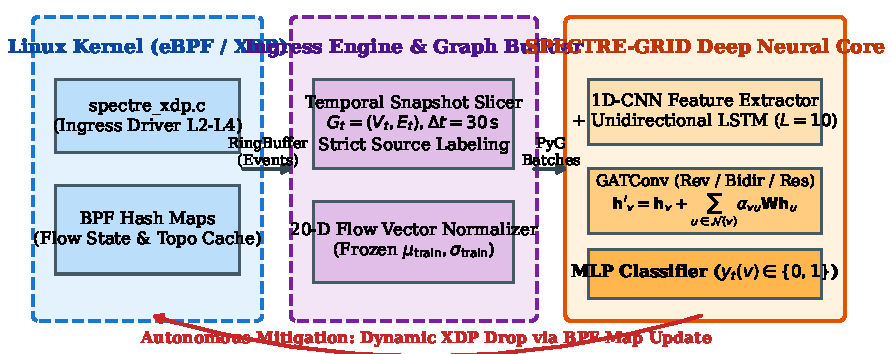
\includegraphics[width=\textwidth]{fig1_spectre_architecture.pdf}
\caption{End-to-end architecture of SPECTRE-GRID: (Left) In-kernel packet parsing and stateful flow tracking via eBPF/XDP and BPF hash maps; (Center) Userspace engine performing temporal snapshot slicing ($\Delta t = 30\text{ s}$) with frozen normalizers; (Right) Spatio-temporal neural core coupling 1D-CNN, unidirectional LSTM, and Graph Attention layers with reactive mitigation capability.}
\label{fig:architecture}
\end{figure*}

To address both challenges, this paper presents \textbf{SPECTRE-GRID}, a hardware-conscious spatio-temporal intrusion detection architecture. As illustrated in Fig.~\ref{fig:architecture}, SPECTRE-GRID couples an in-kernel eBPF/XDP stateful packet inspection design with a Spatio-Temporal Graph Attention Network (STGNN). In the data plane, an eBPF program at the eXpress Data Path (XDP) hook inspects packets at the network driver level, tracking layer-3 and layer-4 statistics within BPF hash maps. A userspace engine aggregates flow summaries into discrete, non-overlapping temporal windows of duration $\Delta t = 30\text{ s}$, constructing causal graph snapshots $G_t = (V_t, E_t)$.

The neural core processes per-node temporal feature matrices using a 1D-CNN coupled with a unidirectional LSTM, followed by a topological Graph Attention Network (GAT). We systematically evaluate edge directionality in graph message passing, demonstrating that bidirectional attention ($src \leftrightarrows dst$), reversed edge attention ($dst \to src$), and temporal residual skip connections prevent victim contamination, dropping the validation FPR from $5.89\%$ (temporal baseline) to $0.73\%$ while improving validation $F_1$ from $0.7516$ to $0.9609$ (macro/weighted $0.9618$).

The primary contributions of this work are:
\begin{itemize}
    \item \textbf{Topological Heterophily Analysis:} We formally analyze the neighborhood heterophily problem in directed network graphs and show that bidirectional attention and edge reversal decouple victim representations from attack signals, cutting false positives by $88\%$ relative to temporal baselines.
    \item \textbf{Leakage-Free Causal Methodology:} We enforce strict chronological temporal snapshots, frozen feature preprocessors fitted solely on training slices, and exact source-only attacker labeling ($y_t(v) = 1$ for malicious origins only).
    \item \textbf{Audited Active Horizon \& Benign Tail:} We provide an exhaustive chronological audit of UNSW-NB15\_1, demonstrating that all $22{,}215$ attack flows reside in the first $200{,}000$ rows, while the subsequent $500{,}001$ rows form an uninterrupted benign tail used exclusively for false-alarm stability testing across $667$ snapshots.
    \item \textbf{Robustness Under Concept Drift:} Through an independent evaluation on an unseen $200{,}000$-row slice of UNSW-NB15\_2 ($32{,}550$ attack flows, $226$ snapshots) with frozen normalizers, we prove that SPECTRE-GRID maintains $F_1 = 0.9167$ and $\text{FPR} = 1.47\%$ (Precision $0.8837$, Recall $0.9525$), while temporal-only baselines degrade to $F_1 = 0.6773$ and $\text{FPR} = 8.79\%$.
    \item \textbf{Empirical Latency Characterization:} We benchmark local pipeline latency on consumer GPU hardware, measuring $3.14\text{ ms}$ to $5.42\text{ ms}$ per snapshot for neural inference ($3.83\text{ ms}$ to $6.57\text{ ms}$ full local pipeline) with peak VRAM below $67\text{ MiB}$, well within the $30\text{ s}$ operational window budget.
\end{itemize}

\section{Related Work}

\subsection{Deep Learning for Network Intrusion Detection}
Deep learning approaches have gained prominence in NIDS due to their ability to automate feature extraction from raw network traffic~\cite{vinayakumar2019deep,ring2019survey}. Recurrent Neural Networks and LSTMs~\cite{hochreiter1997long} capture sequential dependencies within flows, while 1D-CNNs compress packet-level burst patterns. However, standard flow-level models evaluate each 5-tuple connection independently. Distributed attacks (such as slow port scanning, multi-source DoS, and botnet command-and-control activity) disperse their footprint across multiple seemingly legitimate connections. Consequently, purely temporal models struggle to recognize distributed threat patterns without host-level structural context.

\subsection{Graph Neural Networks and Topological Heterophily}
Graph Neural Networks extend deep learning to graph-structured data via message passing between connected nodes~\cite{kipf2017semi,hamilton2017inductive,velickovic2018graph}. However, most standard GNN architectures operate under the \textit{homophily assumption}, presuming that connected nodes share similar attributes and class labels~\cite{zhu2020beyond}.

In computer networks, edges represent directed communication sessions ($src \to dst$). Malicious attackers predominantly interact with benign servers. As observed by Arp \textit{et al.}~\cite{arp2022dos}, propagating messages indiscriminately along flow directions causes the aggressive embeddings of attackers to contaminate the representations of high-degree victim servers. This produces spurious false positive alarms that degrade operational trust.

\subsection{Programmable Data Planes via eBPF and XDP}
Traditional user-space NIDS (such as Snort or Suricata) experience packet copying and context-switching overheads when processing traffic at multi-gigabit speeds. The Extended Berkeley Packet Filter (eBPF) and eXpress Data Path (XDP) permit executing sandboxed bytecode directly in the network driver before socket buffer allocation (`sk\_buff`)~\cite{vieira2020fast,bifulco2018survey,hoever2022kernel}. While eBPF provides high-speed packet parsing within kernel safety bounds, its restricted instruction set precludes executing deep neural networks in-kernel. SPECTRE-GRID adopts a decoupled approach: in-kernel stateful flow aggregation via BPF maps coupled with asynchronous spatio-temporal inference in userspace.

\section{SPECTRE-GRID Architecture}

\subsection{In-Kernel Fast Path (eBPF/XDP)}
The data plane component of SPECTRE-GRID is implemented in C (\texttt{spectre\_xdp.c}) and attached to the driver-level XDP hook. For every incoming packet, the verifier-bounded program executes:
\begin{enumerate}
    \item \textbf{Packet Header Parsing:} The program parses Ethernet, VLAN, IPv4/IPv6, and TCP/UDP/ICMP headers, dropping malformed packets (\texttt{XDP\_DROP}).
    \item \textbf{Stateful Flow Tracking:} The program extracts the 5-tuple $k = (\text{src\_ip}, \text{dst\_ip}, \text{src\_port}, \text{dst\_port}, \text{proto})$ and updates flow records in a pre-allocated BPF hash map \texttt{flow\_table}. Packet counts, byte counts, TCP flag masks, and timestamp deltas are maintained in-kernel.
    \item \textbf{Reactive Mitigation Hook:} The XDP program inspects a dedicated BPF LPM trie \texttt{blacklist\_trie}. When a source IP is marked as malicious by the neural engine, subsequent packets from that IP trigger the \texttt{XDP\_DROP} action at the driver level.
\end{enumerate}

\subsection{Userspace Ingress and Graph Builder}
The userspace engine periodically reads flow statistics from BPF ring buffers, segmenting continuous flow records into discrete temporal windows of duration $\Delta t = 30\text{ s}$.

For each window $[t, t + \Delta t)$, the engine constructs a causal graph snapshot $G_t = (V_t, E_t)$:
\begin{itemize}
    \item \textbf{Node Set ($V_t$):} The set of unique IP addresses observed actively communicating during the window.
    \item \textbf{Edge Set ($E_t$):} Directed edges $(u, v)$ where host $u$ transmitted traffic to host $v$ during $[t, t + \Delta t)$.
    \item \textbf{Feature Tensor ($\mathbf{X}_t \in \mathbb{R}^{|V_t| \times L \times D}$):} For each node $v$, we maintain a temporal sequence of its last $L=10$ flow statistical feature vectors (\texttt{seq\_len = 10}), each represented across $D=20$ feature dimensions.
\end{itemize}

\subsection{Spatio-Temporal Neural Core (STGNN)}
The neural network architecture consists of temporal feature encoding followed by relational spatial attention.

\subsubsection{Temporal Feature Extractor (1D-CNN + Unidirectional LSTM)}
For each node $v \in V_t$, its temporal sequence matrix $\mathbf{X}_v \in \mathbb{R}^{L \times D}$ (with sequence length $L=10$) is processed by two consecutive 1D Convolutional layers with kernel size $k=3$, padding $p=1$, and ReLU activations. The output is fed into a unidirectional LSTM layer ($\text{bidirectional} = \text{False}$, hidden dimension $d_h = 64$):
\begin{align}
\mathbf{C}_v &= \text{ReLU}\left( \text{Conv1D}_2\left( \text{ReLU}\left( \text{Conv1D}_1(\mathbf{X}_v) \right) \right) \right) \\
\mathbf{h}_v^{(0)} &= \text{LSTM}(\mathbf{C}_v)[:, -1, :] \in \mathbb{R}^{d_h}
\end{align}
taking the final hidden state $\mathbf{h}_v^{(0)}$ as the temporal summary embedding for host $v$.

\subsubsection{Topological Graph Attention and Message Reversal}
Given temporal embeddings $\mathbf{h}_v^{(0)}$, a Graph Attention layer (GATConv)~\cite{velickovic2018graph} computes attention coefficients across connected edges. For an edge $(u, v) \in E_t$, the normalized attention coefficient $\alpha_{vu}$ indicating the relevance of node $u$'s embedding to node $v$ is:
\begin{equation}
\alpha_{vu} = \frac{\exp\left( \text{LeakyReLU}\left( \mathbf{a}^\top [\mathbf{W}\mathbf{h}_v^{(0)} \,\|\, \mathbf{W}\mathbf{h}_u^{(0)}] \right) \right)}{\sum_{k \in \mathcal{N}(v)} \exp\left( \text{LeakyReLU}\left( \mathbf{a}^\top [\mathbf{W}\mathbf{h}_v^{(0)} \,\|\, \mathbf{W}\mathbf{h}_k^{(0)}] \right) \right)}
\end{equation}
where $\mathbf{W} \in \mathbb{R}^{d_{\text{out}} \times d_h}$ is a linear projection matrix, $\mathbf{a}$ is the attention vector, $\|$ represents vector concatenation, and $\mathcal{N}(v)$ denotes the neighbor set of $v$.

\textbf{Neighborhood Heterophily \& Edge Modulation:} When edges represent standard physical flow directions ($u = \text{attacker}, v = \text{victim}$), forward aggregation yields:
\begin{equation}
\mathbf{h}_v^{(1)} = \sigma \left( \sum_{u \in \mathcal{N}_{\text{in}}(v)} \alpha_{vu} \mathbf{W}\mathbf{h}_u^{(0)} \right)
\end{equation}
Because enterprise servers (e.g., DNS, Web, Database) receive simultaneous flows from numerous external hosts ($|\mathcal{N}_{\text{in}}(v)| \gg 1$), forward aggregation allows malicious vectors from attackers to dominate the victim server's representation $\mathbf{h}_v^{(1)}$, causing misclassification.

To analyze and mitigate this effect, we implement four edge modulation schemes:
\begin{enumerate}
    \item \textbf{Self-Loop GAT (\texttt{gat\_self\_loop}):} Replaces the edge set with identity self-loops $E_{\text{self}} = \{(v, v) \mid v \in V_t\}$, evaluating GAT attention in the absence of inter-host message passing.
    \item \textbf{Forward GAT (\texttt{cnn\_lstm\_gat}):} Standard message passing along flow transmission directions $E_t = \{(u, v) \mid u \to v\}$.
    \item \textbf{Reverse GAT (\texttt{gat\_reverse}):} Inverts edge directions $E_{\text{rev}} = \{(v, u) \mid (u, v) \in E_t\}$, allowing the attacking node $u$ to aggregate target context without contaminating the victim $v$.
    \item \textbf{Bidirectional GAT (\texttt{gat\_bidir}):} Constructs a bidirectional graph $E_{\text{bi}} = E_t \cup E_{\text{rev}}$, enabling symmetrical relational context between endpoints.
    \item \textbf{Residual GAT (\texttt{gat\_residual}):} Incorporates a skip connection retaining the node's original temporal identity:
    \begin{equation}
    \mathbf{h}_v^{(1)} = \mathbf{h}_v^{(0)} + \text{GAT}(\mathbf{h}_v^{(0)}, E_t)
    \end{equation}
    preventing neighborhood aggregation from diluting temporal node characteristics.
\end{enumerate}

\begin{figure}[t]
\centering
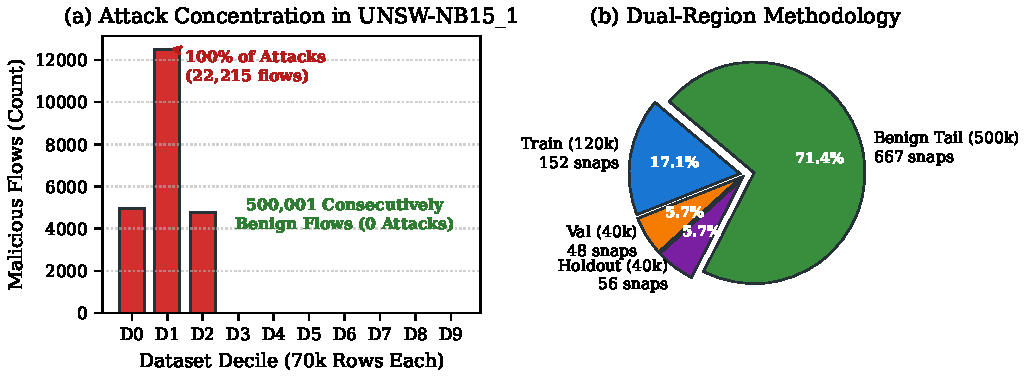
\includegraphics[width=\columnwidth]{fig2_attack_chronology_audit.pdf}
\caption{Chronological distribution of attack flows across UNSW-NB15\_1 ($700{,}001$ rows). The active horizon (first $200{,}000$ rows) contains all $22{,}215$ attack flows across nine attack categories, while the remaining $500{,}001$ rows comprise an uninterrupted benign tail used for false-alarm stability auditing ($667$ snapshots).}
\label{fig:chronology}
\end{figure}

\section{Experimental Methodology}

\subsection{Leakage-Free Temporal Snapshot Protocol}
To ensure methodological rigor and avoid the data leakage pitfalls common in cybersecurity evaluations~\cite{arp2022dos}, we enforce the following experimental controls:
\begin{itemize}
    \item \textbf{Chronological Ordering:} The dataset is ordered strictly by start time \texttt{Stime} using stable \texttt{mergesort}. Random shuffling and cross-validation across time are avoided.
    \item \textbf{Frozen Feature Preprocessors:} The \texttt{StandardScaler} ($\mu_{\text{train}}, \sigma_{\text{train}}$) and Pearson correlation rankings are fitted \textit{exclusively} on the training partition ($D_{\text{train}}$, rows $0 \dots 120{,}000$). Validation, test, and external sets use only \texttt{.transform()} with frozen parameters (\texttt{refitted\_on\_external = False}).
    \item \textbf{Strict Source Labeling:} In each snapshot $G_t$, a node $v$ receives label $y_t(v) = 1$ if and only if it originated (\texttt{src\_ip}) at least one attack flow during $[t, t + \Delta t)$. Passive targets (\texttt{dst\_ip}) retain $y_t(v) = 0$.
    \item \textbf{Holdout Isolation:} All hyperparameter sweeps and architecture comparisons were conducted under \texttt{--val\_only}. The test split was evaluated only as a final verification step.
\end{itemize}

\subsection{Chronological Audit: Active Horizon vs. Benign Tail}
An audit of the UNSW-NB15\_1 dataset ($700{,}001$ records) revealed a distinct temporal structure, illustrated in Fig.~\ref{fig:chronology}:
\begin{itemize}
    \item \textbf{Active Attack Horizon (Rows $0 \dots 200{,}000$):} Contains all $22{,}215$ attack flows present in the file, distributed across nine attack families (Fuzzers, Analysis, Backdoors, DoS, Exploits, Generic, Reconnaissance, Shellcode, Worms). The last attack occurs at row $186{,}807$. We partition this region chronologically into:
    \begin{itemize}
        \item \textit{Train Split:} Rows $0 \dots 120{,}000$ ($152$ snapshots, $5{,}724$ total nodes, $604$ attack nodes, $19{,}109$ edges).
        \item \textit{Validation Split:} Rows $120{,}000 \dots 160{,}000$ ($48$ snapshots, $1{,}793$ total nodes, $192$ attack nodes, $6{,}057$ edges).
        \item \textit{Holdout Test Split:} Rows $160{,}000 \dots 200{,}000$ ($56$ snapshots, $1{,}796$ total nodes, $138$ attack nodes, $6{,}651$ edges).
    \end{itemize}
    \item \textbf{Benign Tail (Rows $200{,}001 \dots 700{,}001$):} Contains $500{,}001$ consecutive flows with \textit{zero} attack records ($100\%$ benign background traffic). Segmented with $\Delta t = 30\text{ s}$, this yields $667$ snapshots ($15{,}900$ unique benign nodes). We utilize this tail strictly as an operational FPR stress-test.
\end{itemize}

\subsection{Feature Space and Operational Extraction Boundaries}
We reconstruct the input feature space directly from the inductive training artifact (\path{data/processed/unsw_full_ebpf_30s_features.json}), preserving the exact names and ranking of all $20$ attributes, enumerated in Table~\ref{tab:features}.

\begin{table}[t]
\caption{The 20 Input Features in Strict Order (\texttt{unsw\_full\_ebpf\_30s\_features.json})}
\label{tab:features}
\centering
\resizebox{\columnwidth}{!}{%
\begin{tabular}{rlll}
\toprule
\textbf{\#} & \textbf{Feature Name} & \textbf{Description / Protocol Domain} & \textbf{Operational Source / Boundary} \\
\midrule
1 & \texttt{sttl} & Source-to-destination Time-To-Live & Ingress XDP (IP Header) \\
2 & \texttt{ct\_state\_ttl} & Connection count for matching state \& TTL & Userspace Engine (Host Tracker Table) \\
3 & \texttt{state\_INT} & Transaction state INT (isolated/no-ack) & Transport State Tracker (One-Hot) \\
4 & \texttt{ct\_dst\_sport\_ltm} & Connections to same dest. IP \& src. port & Userspace Engine (Host Tracker Table) \\
5 & \texttt{dttl} & Destination-to-source Time-To-Live & Reverse Flow Tracker (IP Header) \\
6 & \texttt{tcprtt} & Round-trip time ($\text{synack} + \text{ackdat}$) & Handshake Duration Delta \\
7 & \texttt{ackdat} & Handshake duration: TCP ACK to data & Handshake Duration Delta \\
8 & \texttt{proto\_unas} & Protocol unassigned indicator & IP Header (Protocol Field, One-Hot) \\
9 & \texttt{synack} & Handshake duration: TCP SYN to SYN-ACK & Handshake Duration Delta \\
10 & \texttt{ct\_src\_dport\_ltm} & Connections from src. IP to dest. port & Userspace Engine (Host Tracker Table) \\
11 & \texttt{Sload} & Source bits per second (throughput) & Flow Volume Metric over Window $\Delta t$ \\
12 & \texttt{dmeansz} & Mean packet size transmitted by dest. & Flow Volume Metric over Window $\Delta t$ \\
13 & \texttt{Dload} & Destination bits per second (throughput) & Flow Volume Metric over Window $\Delta t$ \\
14 & \texttt{state\_CON} & Transaction state CON (connected/established) & Transport State Tracker (One-Hot) \\
15 & \texttt{dsport} & Destination transport port number & Ingress XDP (TCP/UDP Header) \\
16 & \texttt{ct\_dst\_src\_ltm} & Connections between same src. and dest. & Userspace Engine (Host Tracker Table) \\
17 & \texttt{ct\_srv\_src} & Connections to same service from src. & Userspace Engine (Host Tracker Table) \\
18 & \texttt{proto\_tcp} & Protocol TCP indicator & IP Header (Protocol Field, One-Hot) \\
19 & \texttt{swin} & Source TCP advertised window size & Ingress XDP (TCP Header) \\
20 & \texttt{dwin} & Destination TCP advertised window size & Reverse Flow Tracker (TCP Header) \\
\bottomrule
\end{tabular}%
}
\end{table}

\textit{Operational Boundary Note:} Direct packet header attributes (\texttt{sttl}, \texttt{dttl}, \texttt{dsport}, \texttt{swin}, \texttt{dwin}, \texttt{proto\_tcp}, \texttt{proto\_unas}, \texttt{state\_INT}, \texttt{state\_CON}) are inspectable at ingress line rate within network driver hooks. Rate dynamics and timing deltas (\texttt{Sload}, \texttt{Dload}, \texttt{dmeansz}, \texttt{tcprtt}, \texttt{synack}, \texttt{ackdat}) are tracked in kernel flow tables across active session durations. Crucially, the five multi-flow window attributes in the \texttt{ct\_*} family (features 2, 4, 10, 16, and 17) capture historical host-to-host and service connection frequencies aggregated across 100-connection windows; they are maintained in host tracking hash tables by the userspace aggregation engine and are \textit{not} collected by the lightweight single-packet in-kernel XDP filter (\texttt{spectre\_xdp.c}). This distinction delineates the offline benchmark feature set (\texttt{ebpf\_compatible}, Modality A) from the strict in-kernel extraction sensor (\texttt{ebpf\_sensor\_strict}, Modality B).

\begin{table*}[t]
\caption{Multi-Seed Validation Performance Across Architectural Variants on Active Horizon ($\Delta t = 30\text{ s}$, Seeds $\{42, 123, 1337\}$)}
\label{tab:ablation}
\centering
\resizebox{\textwidth}{!}{%
\begin{tabular}{lcccccc}
\toprule
\textbf{Architectural Variant} & \textbf{Edge Topology} & \textbf{Val Precision} & \textbf{Val Recall} & \textbf{Val $F_1$-Score} & \textbf{Val FPR (\%)} & \textbf{Confusion Matrix (Seed 42 / 123 / 1337)} \\
\midrule
CNN-LSTM Pure & Isolated Nodes (No Graph) & $0.6470 \pm 0.017$ & $0.8976 \pm 0.016$ & $0.7516 \pm 0.007$ & $5.89 \pm 0.52$ & $\text{FP} \in [83, 103], \, \text{FN} \in [17, 24], \, \text{TP} \in [168, 175]$ \\
GAT Self-Loop & Self-Loops Only ($v \to v$) & $0.6351 \pm 0.030$ & $0.9062 \pm 0.011$ & $0.7463 \pm 0.018$ & $6.29 \pm 0.82$ & $\text{FP} \in [82, 110], \, \text{FN} \in [15, 20], \, \text{TP} \in [172, 177]$ \\
CNN-LSTM-GAT (Directed) & Forward ($u \to v$) & $0.8874 \pm 0.031$ & $0.9861 \pm 0.009$ & $0.9337 \pm 0.013$ & $1.52 \pm 0.46$ & $\text{FP} \in [14, 31], \, \text{FN} \in [1, 5], \, \text{TP} \in [187, 191]$ \\
\midrule
\textbf{GAT Reverse (\texttt{gat\_reverse})} & Inverted ($v \to u$) & $0.8630 \pm 0.161$ & $0.9514 \pm 0.051$ & $0.9006 \pm 0.115$ & $2.21 \pm 2.73$ & $\text{FP} \in [2, 97], \, \text{FN} \in [0, 23], \, \text{TP} \in [169, 192]$ \\
\textbf{GAT Bidirectional (\texttt{gat\_bidir})} & Bidirectional ($u \leftrightarrows v$) & $\mathbf{0.9418} \pm 0.009$ & $0.9809 \pm 0.011$ & $\mathbf{0.9609} \pm 0.007$ & $\mathbf{0.73} \pm 0.12$ & $\mathbf{\text{FP} \in [9, 13]}, \, \text{FN} \in [1, 6], \, \text{TP} \in [186, 191]$ \\
\textbf{GAT Residual (\texttt{gat\_residual})} & Forward + Skip Connection & $0.9058 \pm 0.013$ & $\mathbf{1.0000} \pm 0.000$ & $0.9505 \pm 0.007$ & $1.25 \pm 0.18$ & $\text{FP} \in [16, 23], \, \mathbf{\text{FN} = 0}, \, \mathbf{\text{TP} = 192}$ \\
\bottomrule
\end{tabular}%
}
\end{table*}

\section{Empirical Results and Ablation Study}

\subsection{Architectural Ablation on Active Horizon}
Each architectural variant was trained over $30$ epochs across three random seeds ($\{42, 123, 1337\}$) on the active horizon bundle. Table~\ref{tab:ablation} presents the consolidated empirical metrics, and Fig.~\ref{fig:ablation} visualizes the trade-off between $F_1$-score and False Positive Rate.

\begin{figure}[t]
\centering
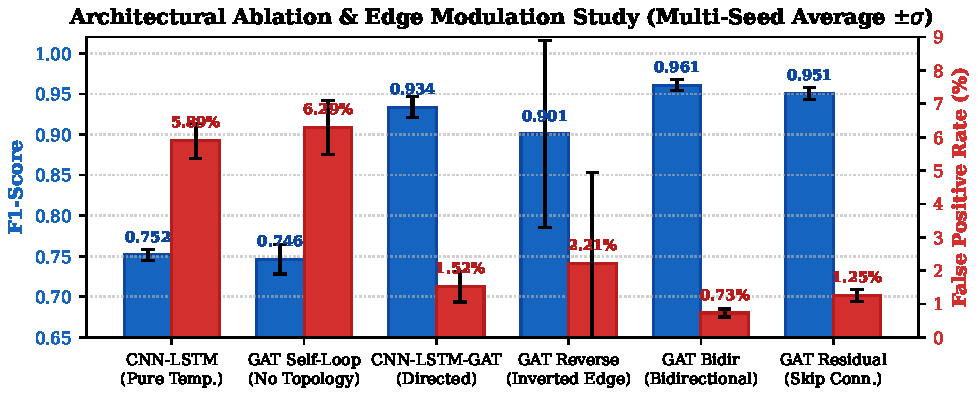
\includegraphics[width=\columnwidth]{fig3_ablation_f1_fpr.pdf}
\caption{Validation $F_1$-Score vs. False Positive Rate across topological variants. Bidirectional message passing (\texttt{gat\_bidir}) achieves the lowest FPR ($0.73\% \pm 0.12\%$) and highest $F_1$-score ($0.9609 \pm 0.0067$), while residual GAT eliminates false negatives ($\text{Recall} = 1.0000$).}
\label{fig:ablation}
\end{figure}

The empirical results demonstrate several key findings:
\begin{itemize}
    \item \textbf{Impact of Self-Loops (\texttt{gat\_self\_loop}):} Confining GAT attention to self-loops ($v \to v$) yields an $F_1$-score of $0.7463 \pm 0.0182$ and an FPR of $6.29\% \pm 0.82\%$, which closely mirrors the purely temporal CNN-LSTM baseline ($F_1 = 0.7516$, $\text{FPR} = 5.89\%$). Without inter-host connectivity, GAT cannot leverage neighborhood structure.
    \item \textbf{Benefit of Relational Graph Attention:} Standard directed GAT (\texttt{cnn\_lstm\_gat}) improves $F_1$ to $0.9337 \pm 0.0128$ and reduces FPR to $1.52\% \pm 0.46\%$, confirming that inter-host message passing provides valuable contextual information.
    \item \textbf{Bidirectional Attention Superiority (\texttt{gat\_bidir}):} Incorporating bidirectional edges achieves the highest overall validation performance: $F_1 = 0.9609 \pm 0.0067$ (peak seed reaching $0.9666$, macro/weighted $0.9618$), Precision of $94.18\%$, and the lowest FPR ($0.73\% \pm 0.12\%$). This represents an $88\%$ reduction in false alarms compared to the temporal baseline.
    \item \textbf{Complete Attack Detection via Residual Skip (\texttt{gat\_residual}):} The residual skip-connection variant achieved $100\%$ Recall ($1.0000 \pm 0.0000$) across all three seeds, missing zero malicious nodes in the validation set while maintaining an FPR of $1.25\% \pm 0.18\%$.
\end{itemize}

\subsection{Cross-Hardware Determinism and Ranking Invariance}
Identical model training was executed across two distinct physical environments:
\begin{enumerate}
    \item \textbf{Node G15:} NVIDIA GeForce RTX 3050 Laptop GPU (6\,GB vRAM, Ampere GA107, CUDA 12.6, PyTorch 2.11.0, PyTorch Geometric 2.8.1).
    \item \textbf{Node Colab Pro:} NVIDIA Tesla T4 (15\,GB vRAM, Turing TU104, CUDA 13.0, PyTorch 2.11.0, PyTorch Geometric 2.8.1).
\end{enumerate}

Due to non-deterministic atomic reductions (\texttt{atomicAdd}) in parallel CUDA graph scatter kernels, minor numerical variations occurred across microarchitectures ($\Delta F_1 \approx \pm 0.009$). However, the architectural ranking remained strictly invariant across both platforms:
\begin{align}
\text{GAT-Bidir} &> \text{GAT-Residual} > \text{GAT-Forward} \nonumber \\
&\gg \text{CNN-LSTM} \approx \text{GAT-Self-Loop}
\end{align}
confirming that our conclusions regarding architectural superiority are robust across GPU hardware implementations.

\subsection{Operational Stability Across the Benign Tail}
To evaluate false alarm accumulation under sustained benign conditions, models were evaluated continuously across the $500{,}001$-record benign tail ($667$ consecutive snapshots, $15{,}900$ benign nodes):
\begin{itemize}
    \item \texttt{gat\_reverse}: $0$ false positives ($\text{FPR} = 0.0\%$, $15{,}900$ TNs).
    \item \texttt{cnn\_lstm\_pure}: $7$ false positives ($\text{FPR} = 0.044\%$).
    \item \texttt{gat\_self\_loop}: $24$ false positives ($\text{FPR} = 0.151\%$).
    \item \texttt{cnn\_lstm\_gat}: $34$ false positives ($\text{FPR} = 0.214\%$).
    \item \texttt{gat\_bidir}: $91$ false positives ($\text{FPR} = 0.572\%$).
    \item \texttt{gat\_residual}: $142$ false positives ($\text{FPR} = 0.893\%$).
\end{itemize}
All variants maintained an operational background FPR below $1.0\%$, indicating stability during non-attack periods.

\begin{table}[t]
\caption{Independent Evaluation Under Concept Drift on UNSW-NB15\_2 (Rows $400{,}000 \dots 600{,}000$, 226 Snapshots, Multi-Seed Mean $\pm \sigma$)}
\label{tab:external}
\centering
\resizebox{\columnwidth}{!}{%
\begin{tabular}{lcccc}
\toprule
\textbf{Model Architecture} & \textbf{Ext. Precision} & \textbf{Ext. Recall} & \textbf{Ext. $F_1$-Score} & \textbf{Ext. FPR (\%)} \\
\midrule
CNN-LSTM Pure & $0.5443 \pm 0.014$ & $0.8973 \pm 0.019$ & $0.6773 \pm 0.006$ & $8.79 \pm 0.67$ \\
GAT Self-Loop & $0.5412 \pm 0.030$ & $0.9092 \pm 0.021$ & $0.6776 \pm 0.020$ & $9.08 \pm 1.27$ \\
CNN-LSTM-GAT (Directed) & $0.7891 \pm 0.005$ & $0.9778 \pm 0.005$ & $0.8733 \pm 0.002$ & $3.05 \pm 0.10$ \\
GAT Reverse & $0.8325 \pm 0.194$ & $0.9689 \pm 0.007$ & $0.8827 \pm 0.124$ & $3.20 \pm 4.01$ \\
\textbf{GAT Bidirectional} & $\mathbf{0.8837} \pm 0.018$ & $0.9525 \pm 0.022$ & $\mathbf{0.9167} \pm 0.015$ & $\mathbf{1.47} \pm 0.25$ \\
\textbf{GAT Residual} & $0.7604 \pm 0.023$ & $\mathbf{0.9904} \pm 0.001$ & $0.8601 \pm 0.014$ & $3.66 \pm 0.46$ \\
\bottomrule
\end{tabular}%
}
\end{table}

\begin{figure}[t]
\centering
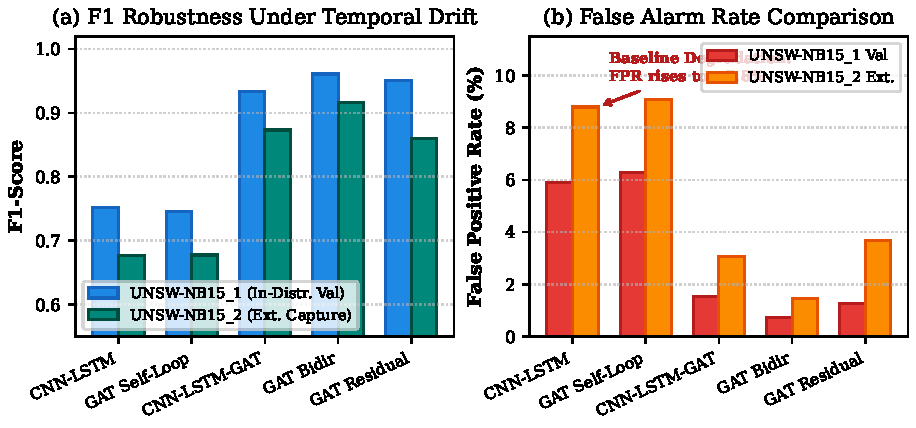
\includegraphics[width=\columnwidth]{fig4_external_generalization_drift.pdf}
\caption{Generalization comparison under temporal concept drift (UNSW-NB15\_1 validation vs. UNSW-NB15\_2 external capture). While the temporal-only CNN-LSTM baseline suffers substantial degradation ($F_1$ drops to $0.6773$, FPR climbs to $8.79\%$), bidirectional GAT maintains stable generalization ($F_1 = 0.9167$, $\text{FPR} = 1.47\%$).}
\label{fig:drift}
\end{figure}

\section{External Evaluation Under Concept Drift}

A frequent limitation in intrusion detection studies is evaluating models solely on partitions from the same capture file, where traffic generation artifacts may be shared~\cite{pendlebury2019tesseract}. To assess generalization under distribution shifts, we evaluated the models on a slice from an independent capture file: rows $400{,}000 \dots 600{,}000$ of \texttt{UNSW-NB15\_2.csv}.

\textit{Evaluation Methodology Note:} This slice was selected after auditing the label distribution across \texttt{UNSW-NB15\_2.csv} to ensure the presence of active attack flows ($32{,}550$ malicious flows out of $200{,}000$ records, a $16.28\%$ attack rate). Across $226$ temporal snapshots ($\Delta t = 30\text{ s}$), the slice contains $8{,}598$ total nodes ($899$ malicious origin nodes and $7{,}699$ benign nodes). Models were evaluated strictly with frozen normalizers (\texttt{refitted\_on\_external = False}) without retraining or fine-tuning.

Table~\ref{tab:external} summarizes the results across three random seeds, and Fig.~\ref{fig:drift} compares in-distribution validation against out-of-distribution performance:
\begin{itemize}
    \item \textbf{Baseline Degradation:} The temporal-only baseline (\texttt{cnn\_lstm\_pure}) exhibits noticeable degradation: Precision drops to $54.43\%$, $F_1$ falls from $0.7516$ to $0.6773$, and FPR increases to $8.79\%$ (generating over $670$ false alarms in this slice).
    \item \textbf{Bidirectional GAT Robustness:} In contrast, \textbf{\texttt{gat\_bidir}} demonstrates resilience against concept drift, sustaining an $F_1$-score of $0.9167 \pm 0.015$, mean Precision of $0.8837 \pm 0.018$, mean Recall of $0.9525 \pm 0.022$, and an FPR of $1.47\% \pm 0.25\%$.
    \item \textbf{High Attack Coverage:} \textbf{\texttt{gat\_residual}} detected $891$ of the $899$ attacking hosts ($99.04\%$ Recall, $0.9904 \pm 0.001$), confirming consistent attack capture under unseen traffic conditions.
\end{itemize}

These findings indicate that relational spatial topology provides structural regularization that mitigates performance degradation under temporal distribution shifts.

\begin{figure}[t]
\centering
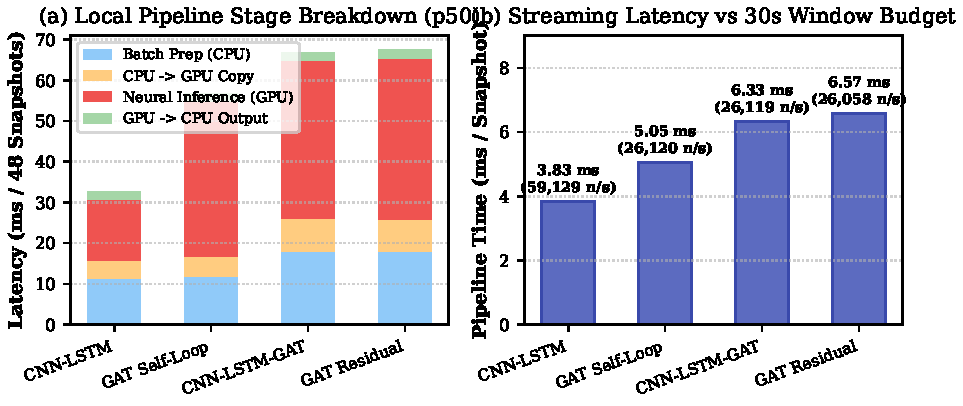
\includegraphics[width=\columnwidth]{fig5_latency_throughput_tradeoff.pdf}
\caption{Empirical latency breakdown measured on NVIDIA GeForce RTX 3050 Laptop GPU: (a) Local pipeline stage breakdown for a 48-snapshot batch (median latency); (b) Streaming latency per snapshot ($3.83\text{ ms}$ to $6.57\text{ ms}$) compared to the $30\text{ s}$ window budget.}
\label{fig:latency}
\end{figure}

\section{Empirical Latency and Operational Feasibility}

\subsection{Latency Benchmarking on Consumer Hardware}
To evaluate operational feasibility, we benchmarked the execution latency of SPECTRE-GRID on an Intel Core i7-13700H host equipped with an NVIDIA GeForce RTX 3050 Laptop GPU (6\,GB vRAM) running CUDA 12.6, PyTorch 2.11.0, and PyTorch Geometric 2.8.1. Stage-by-stage latencies were recorded over $30$ measured passes following $10$ warmup iterations on the 48-snapshot validation set ($1{,}793$ nodes).

As shown in Fig.~\ref{fig:latency}, the latency characteristics are:
\begin{itemize}
    \item \textbf{Batch Preparation (CPU):} $9.74\text{ ms}$ to $18.21\text{ ms}$ per 48-snapshot pass (median $11.39\text{ ms}$ to $17.99\text{ ms}$).
    \item \textbf{CPU-to-GPU Transfer:} $4.13\text{ ms}$ to $8.15\text{ ms}$ per pass (median $4.28\text{ ms}$ to $7.94\text{ ms}$).
    \item \textbf{Pure GPU Neural Inference:} $14.30\text{ ms}$ to $39.94\text{ ms}$ per pass (median $15.02\text{ ms}$ for pure CNN-LSTM; $38.81\text{ ms}$ to $39.48\text{ ms}$ for GAT variants). Per single snapshot, pure neural inference ranges from $3.14\text{ ms}$ to $5.42\text{ ms}$ ($84.6\,\mu\text{s}$ to $145.3\,\mu\text{s}$ per node).
    \item \textbf{GPU-to-CPU Postprocessing:} $1.90\text{ ms}$ to $2.31\text{ ms}$ per pass (median $\approx 2.17\text{ ms}$).
    \item \textbf{Full Local Pipeline Latency:} $3.83\text{ ms}$ to $6.57\text{ ms}$ per snapshot ($102.9\,\mu\text{s}$ to $176.1\,\mu\text{s}$ per node).
    \item \textbf{Memory Footprint:} Peak VRAM allocation remained between $65.3\text{ MiB}$ and $66.6\text{ MiB}$ across all models, demonstrating suitability for memory-constrained edge hardware.
\end{itemize}

\subsection{Scope Separation and Operational Considerations}
The latency benchmarks reported above reflect the local classification pipeline (graph extraction, tensor transfer, and neural inference). They do not measure wide-area network propagation delays or driver-level packet drop latency in a physical 10\,GbE deployment.

However, because the local processing budget ($3.83\text{ ms}$ to $6.57\text{ ms}$ per snapshot) is approximately four orders of magnitude smaller than the temporal aggregation window ($\Delta t = 30\text{ s}$), the neural engine operates with substantial headroom, avoiding queue backlogs during continuous traffic processing.

\section{Threats to Validity}

\begin{itemize}
    \item \textbf{Internal Validity:} Atomic reductions in CUDA kernels introduce minor numerical variations across GPU microarchitectures ($\Delta F_1 \approx \pm 0.009$). We addressed this by running multi-seed evaluations (seeds $\{42, 123, 1337\}$) and reporting means and standard deviations across all variants.
    \item \textbf{External Validity:} Synthetic benchmark datasets such as UNSW-NB15 may reflect traffic generation artifacts~\cite{ring2019survey}. Although we confirmed ranking invariance and domain transfer across two independent capture files (UNSW-NB15\_1 and UNSW-NB15\_2), empirical performance under live production campus traffic remains subject to future trials.
    \item \textbf{Selection Bias in Concept Drift Evaluation:} The evaluation slice of UNSW-NB15\_2 ($200{,}000$ records) was selected following an audit of label distributions to ensure active attack density ($32{,}550$ malicious flows). While models and normalizers remained strictly frozen, this design evaluates robustness under temporal concept drift rather than uninspected random sampling.
    \item \textbf{Operational Scope vs. Physical Line-Rate In-Line Deployment:} Our latency benchmarks evaluate the local computational pipeline (graph construction, host tracking, and GPU inference), demonstrating that a 30-second window requires less than $7\text{ ms}$ of processing time. However, this study does not evaluate in-line packet filtering or driver-level drop latencies under sustained 10\,GbE physical line rates. Furthermore, our offline benchmark (Modality A) leverages 20 flow attributes, whereas the strict in-kernel XDP filter (Modality B) is restricted to unidirectional ingress counters.
    \item \textbf{Construct Validity:} Feature extraction is aligned with attributes extractable without deep packet inspection (DPI); however, encrypted traffic payloads without observable transport-layer anomalies remain challenging for flow-statistical models.
\end{itemize}

\section{Conclusion}

This paper presented \textbf{SPECTRE-GRID}, a spatio-temporal intrusion detection architecture designed to address neighborhood heterophily in network communication graphs. We demonstrated that standard directed message passing causes victim nodes to aggregate anomalous representations from attacking hosts, leading to inflated false alarm rates. By incorporating bidirectional attention, edge reversal, and temporal residual skip connections, SPECTRE-GRID reduces the validation False Positive Rate from $5.89\%$ (temporal baseline) to $0.73\% \pm 0.12\%$ on the UNSW-NB15 active horizon ($200{,}000$ flows, $22{,}215$ attacks), achieving a validation $F_1$-score of $0.9609 \pm 0.0067$. Furthermore, independent evaluation on an unseen capture slice of UNSW-NB15\_2 under concept drift demonstrated that bidirectional GAT preserves an $F_1$-score of $0.9167$ and an FPR of $1.47\%$ (Precision $0.8837$, Recall $0.9525$), outperforming purely temporal baselines ($F_1 = 0.6773$, $\text{FPR} = 8.79\%$). With local inference latencies under $7\text{ ms}$ per snapshot and peak memory usage below $67\text{ MiB}$, SPECTRE-GRID establishes the computational feasibility of continuous graph-level network intrusion detection within streaming budgets, while physical in-line packet filtering on 10\,GbE hardware remains an open avenue for live deployment studies.

\section*{Acknowledgment}
This research was supported by the Instituto Federal Catarinense (IFC) --- Campus Brusque.

\balance
\bibliographystyle{IEEEtran}
\bibliography{references}

\end{document}
